% ------------------------------------------------------------------------------
% TYPO3 CMS 8.5 - What's New - Chapter "Backend User Interface" (French Version)
%
% @author	Michael Schams <schams.net>
% @license	Creative Commons BY-NC-SA 3.0
% @link		http://typo3.org/download/release-notes/whats-new/
% @language	French
% ------------------------------------------------------------------------------
% LTXE-CHAPTER-UID:		07b25346-95b1df21-a6ebe09a-49f53f41
% LTXE-CHAPTER-NAME:	Interface Utilisateur Backend
% ------------------------------------------------------------------------------

\section{Interface Utilisateur Backend}
\begin{frame}[fragile]
	\frametitle{Interface Utilisateur Backend}

	\begin{center}\huge{Chapitre 1~:}\end{center}
	\begin{center}\huge{\color{typo3darkgrey}\textbf{Interface Utilisateur Backend}}\end{center}

\end{frame}

% ------------------------------------------------------------------------------
% LTXE-SLIDE-START
% LTXE-SLIDE-UID:		e00709d6-ccb8a4d0-1cca1d28-431a00a5
% LTXE-SLIDE-TITLE:		#77910: New Form Framework (1)
% ------------------------------------------------------------------------------
\begin{frame}[fragile]
	\frametitle{Interface Utilisateur Backend}
	\framesubtitle{Nouveau framework de formulaires (1)}

	\begin{itemize}
		\item Un nouveau framework flexible de formulaire pour la composition de
			formulaires est intégré dans TYPO3 CMS 8.5
		\item Il remplace l'ancien \textit{Assistant Formulaire} basé sur ExtJS et
			dépendant du système de rendu Frontend
		\item Le nouvel \textit{Éditeur de Formulaire} utilise jQuery et une architecture
			moderne, garantissant flexibilité et extensibilité
		\item Très personnalisable. Les options de configuration sont enregistrées dans des fichiers YAML
		\item La liste des fonctionnalités est impressionnante\newline
			\small(restez à l'écoute pour la documentation complète)\normalsize
		\item Une vidéo de démonstration est disponible sur YouTube~:\newline
			\url{https://www.youtube.com/watch?v=F9sTAOEcTI0}
	\end{itemize}

\end{frame}
% ------------------------------------------------------------------------------
% LTXE-SLIDE-START
% LTXE-SLIDE-UID:		3bbca669-629eab1c-0230fd06-71e7071c
% LTXE-SLIDE-TITLE:		#77910: New Form Framework (2)
% ------------------------------------------------------------------------------
\begin{frame}[fragile]
	\frametitle{Interface Utilisateur Backend}
	\framesubtitle{Nouveau framework de formulaires (2)}

	\begin{figure}
		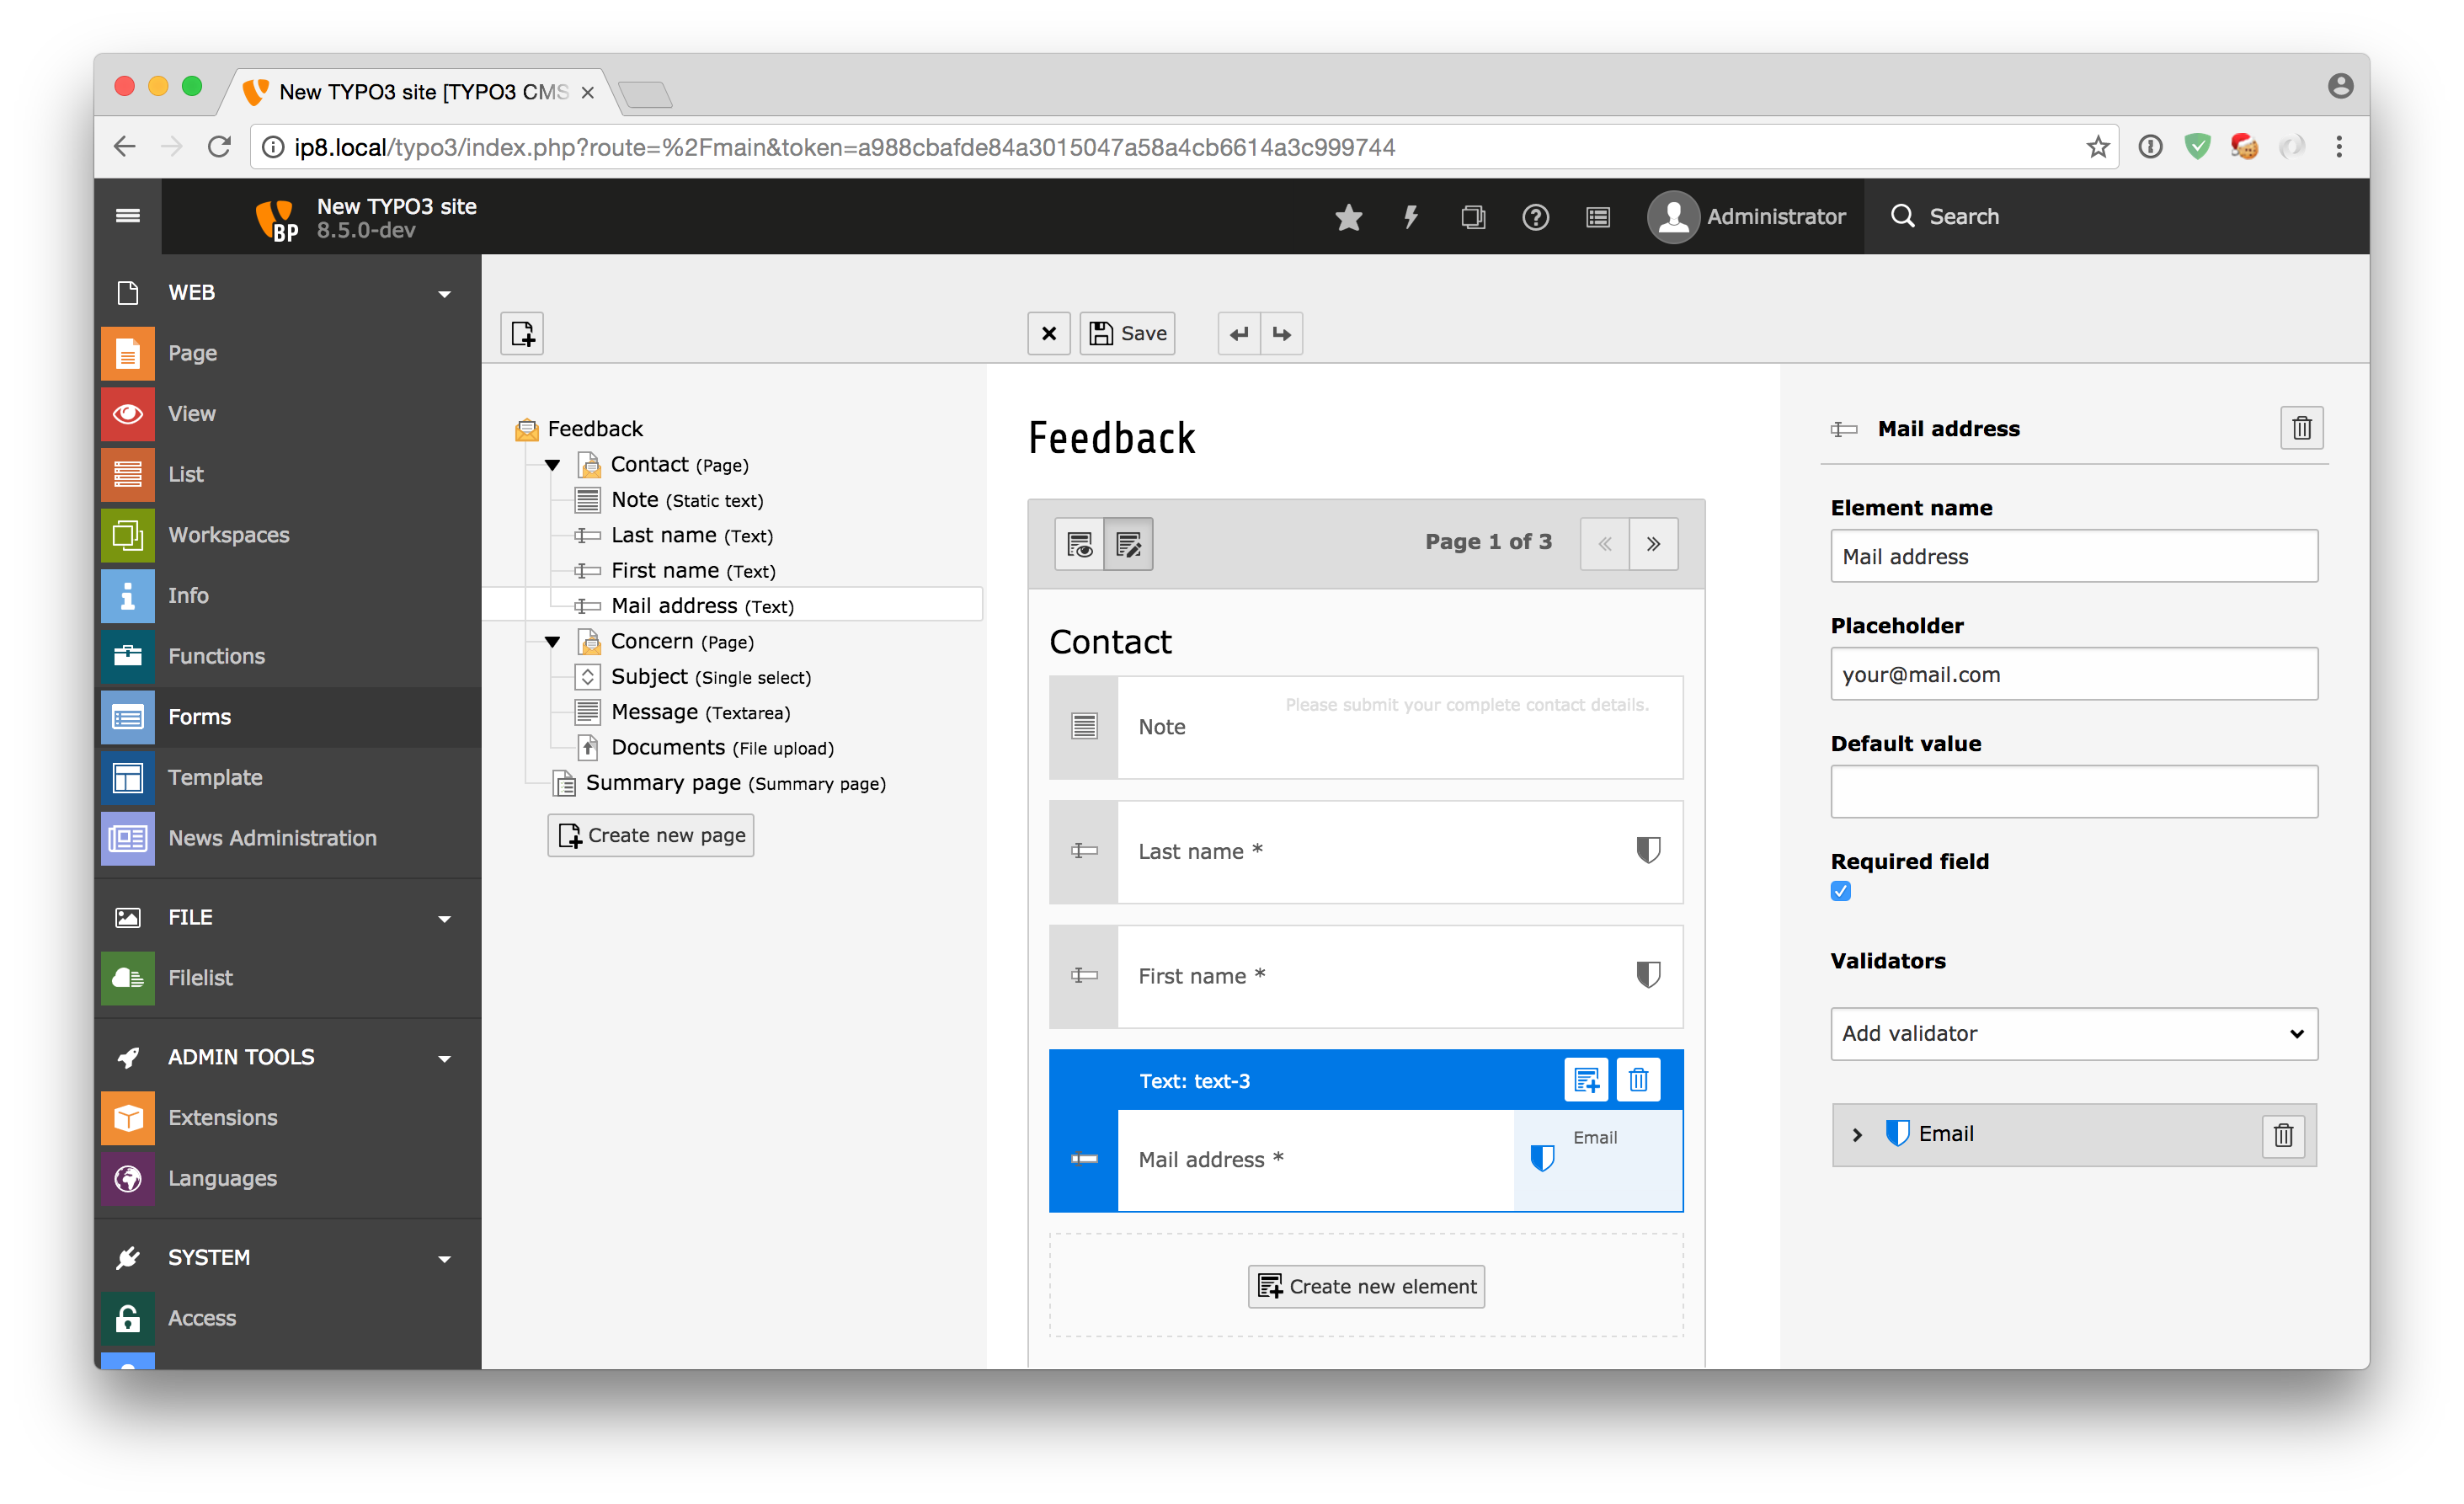
\includegraphics[width=0.8\linewidth]{BackendUserInterface/form-framework-1.png}
	\end{figure}

\end{frame}

% ------------------------------------------------------------------------------
% LTXE-SLIDE-START
% LTXE-SLIDE-UID:		b91ec75b-7aa7b566-b523ca5f-f9ba3cde
% LTXE-SLIDE-TITLE:		#77910: New Form Framework (3)
% ------------------------------------------------------------------------------
\begin{frame}[fragile]
	\frametitle{Interface Utilisateur Backend}
	\framesubtitle{Nouveau Framework de formulaires (3)}

	\begin{figure}
		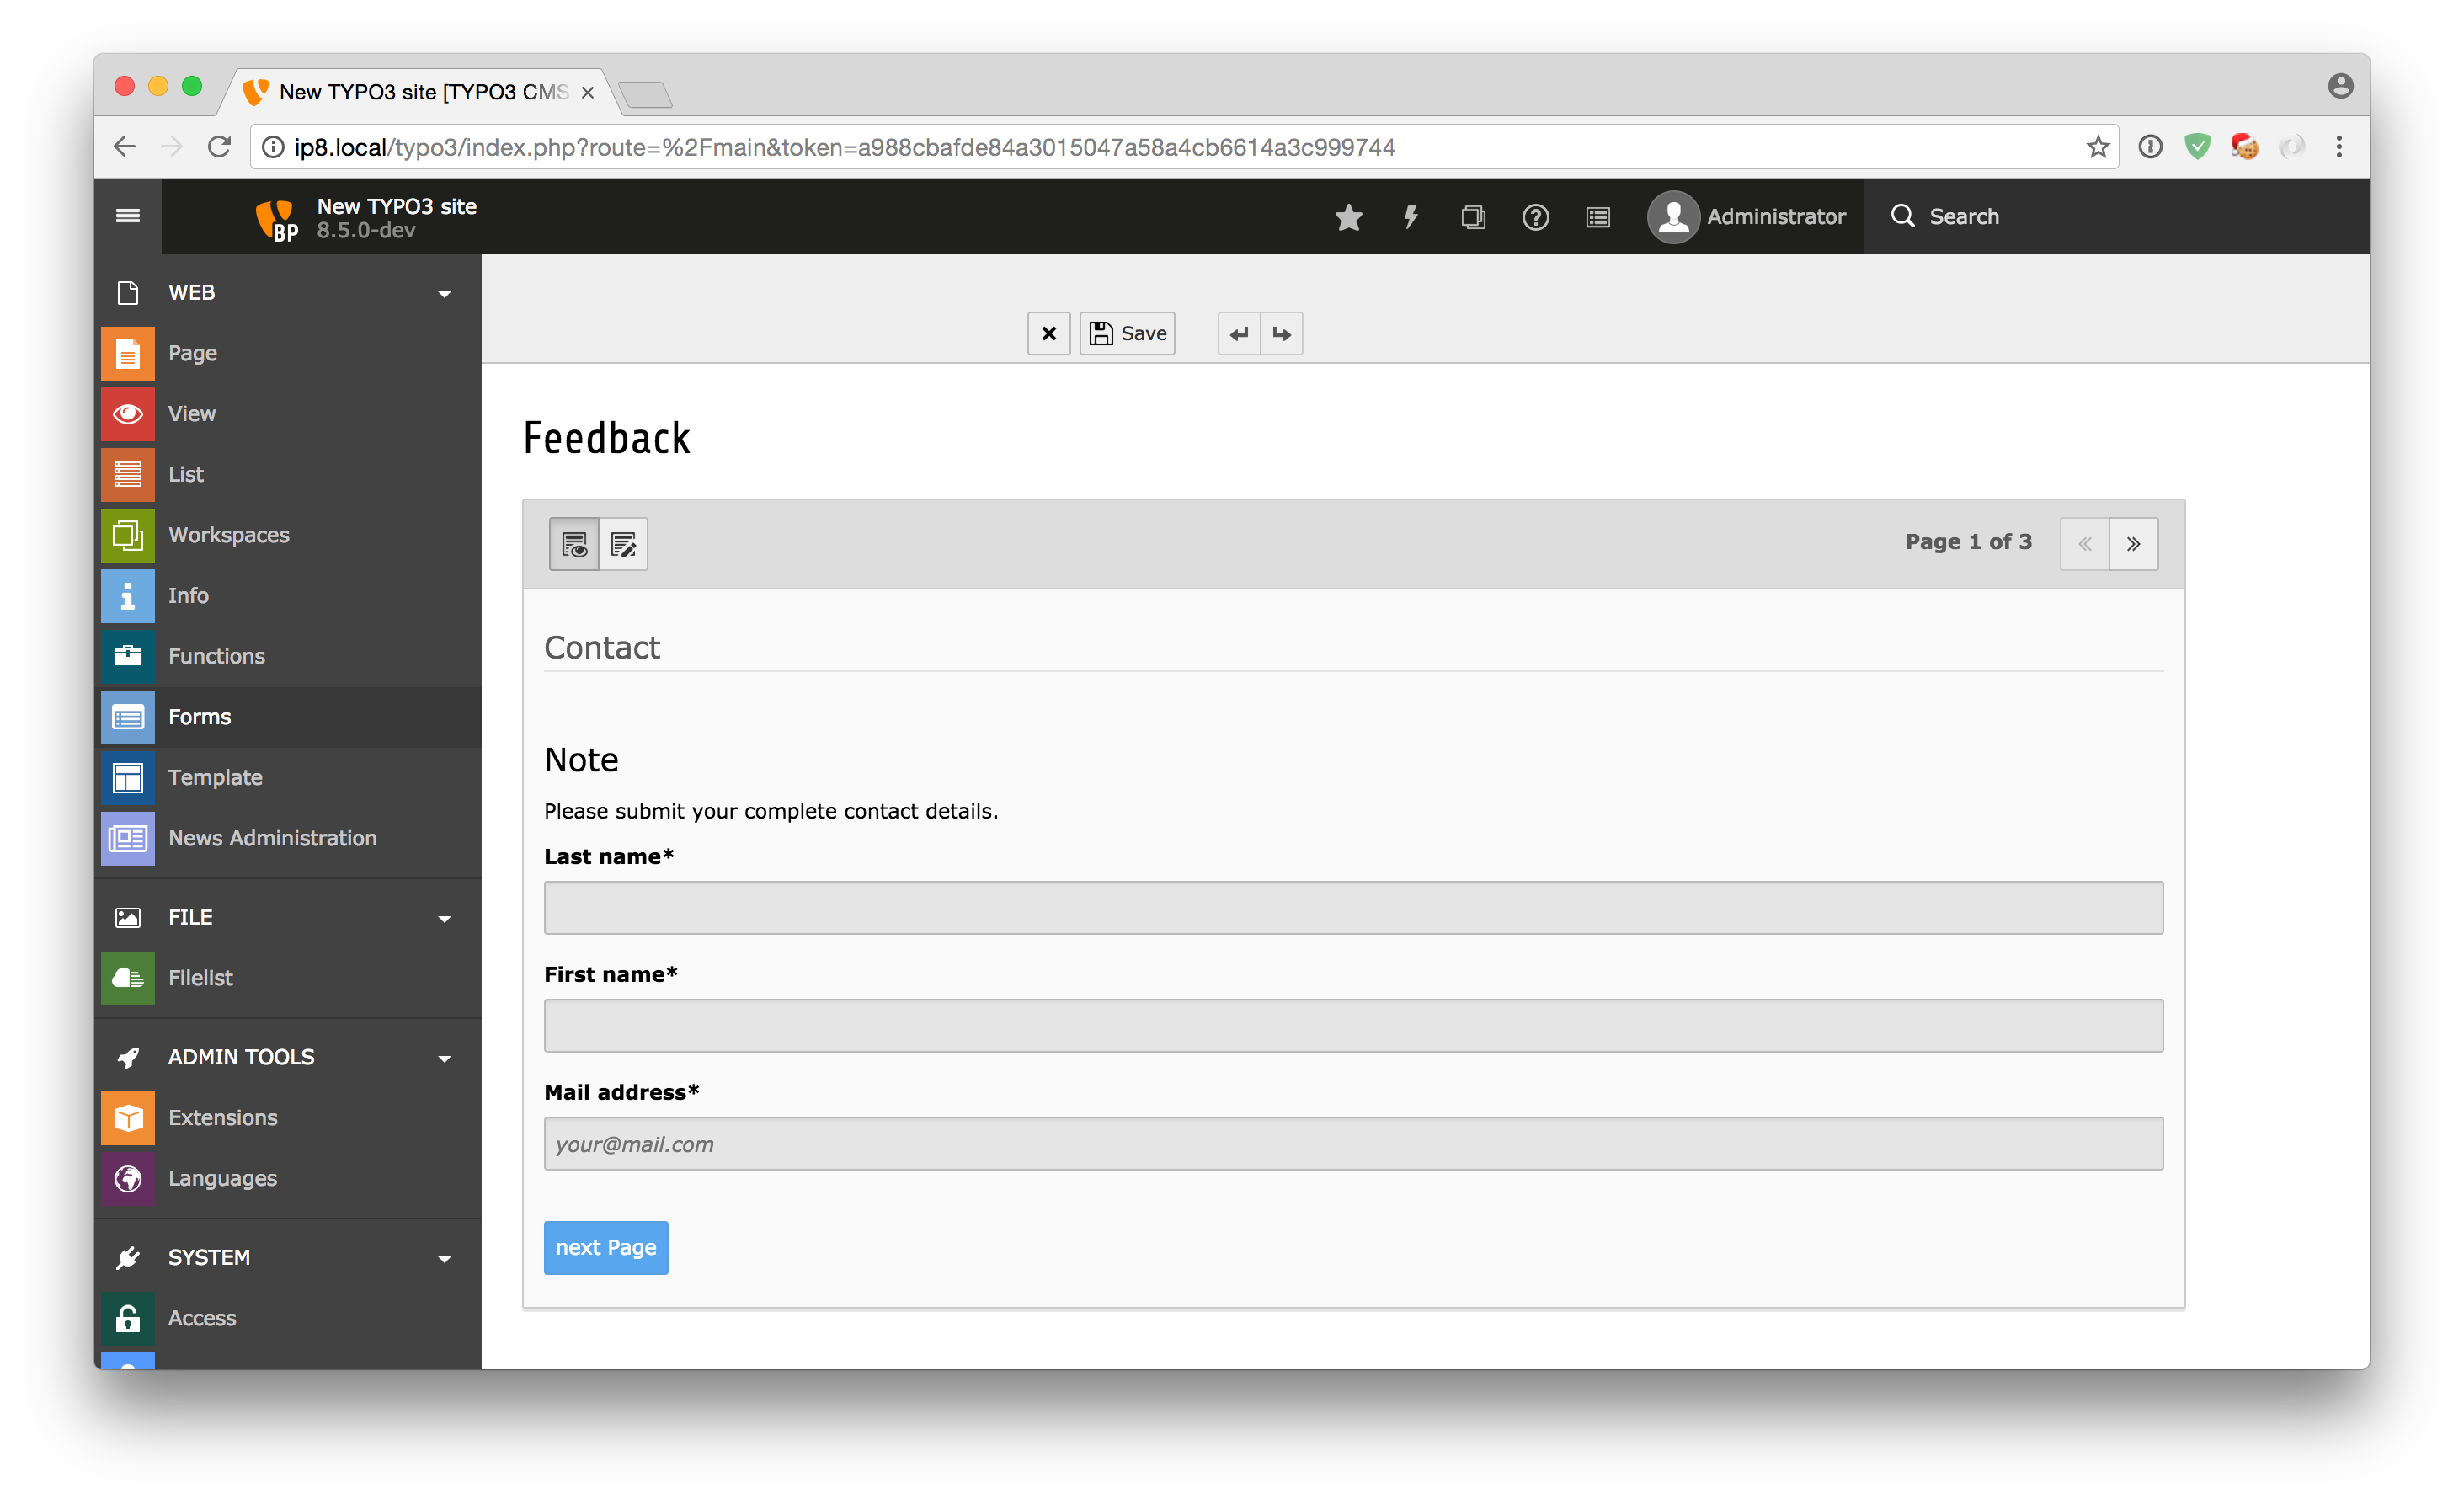
\includegraphics[width=0.8\linewidth]{BackendUserInterface/form-framework-2.png}
	\end{figure}

\end{frame}


% ------------------------------------------------------------------------------
% LTXE-SLIDE-START
% LTXE-SLIDE-UID:		c41b2f21-fb92bb80-56e7ddc9-1c725e34
% LTXE-SLIDE-TITLE:		CKEditor Integration
% ------------------------------------------------------------------------------
\begin{frame}[fragile]
	\frametitle{Interface Utilisateur Backend}
	\framesubtitle{Intégration de CKEditor}

	\begin{columns}[T]
		\begin{column}{.5\textwidth}
			La nouvelle génération d'éditeur de texte riche est implémenté dans le backend TYPO3~:
			\textbf{CKEditor}.\newline

			L'état actuel est marqué explicitement \textit{expérimental} et l'extension
			n'est pas installée par défaut.\newline

			Plus d'informations sur cet éditeur open-source~: \url{http://ckeditor.com}
		\end{column}
		\begin{column}{.5\textwidth}
			\begin{figure}\vspace*{-0.4cm}
				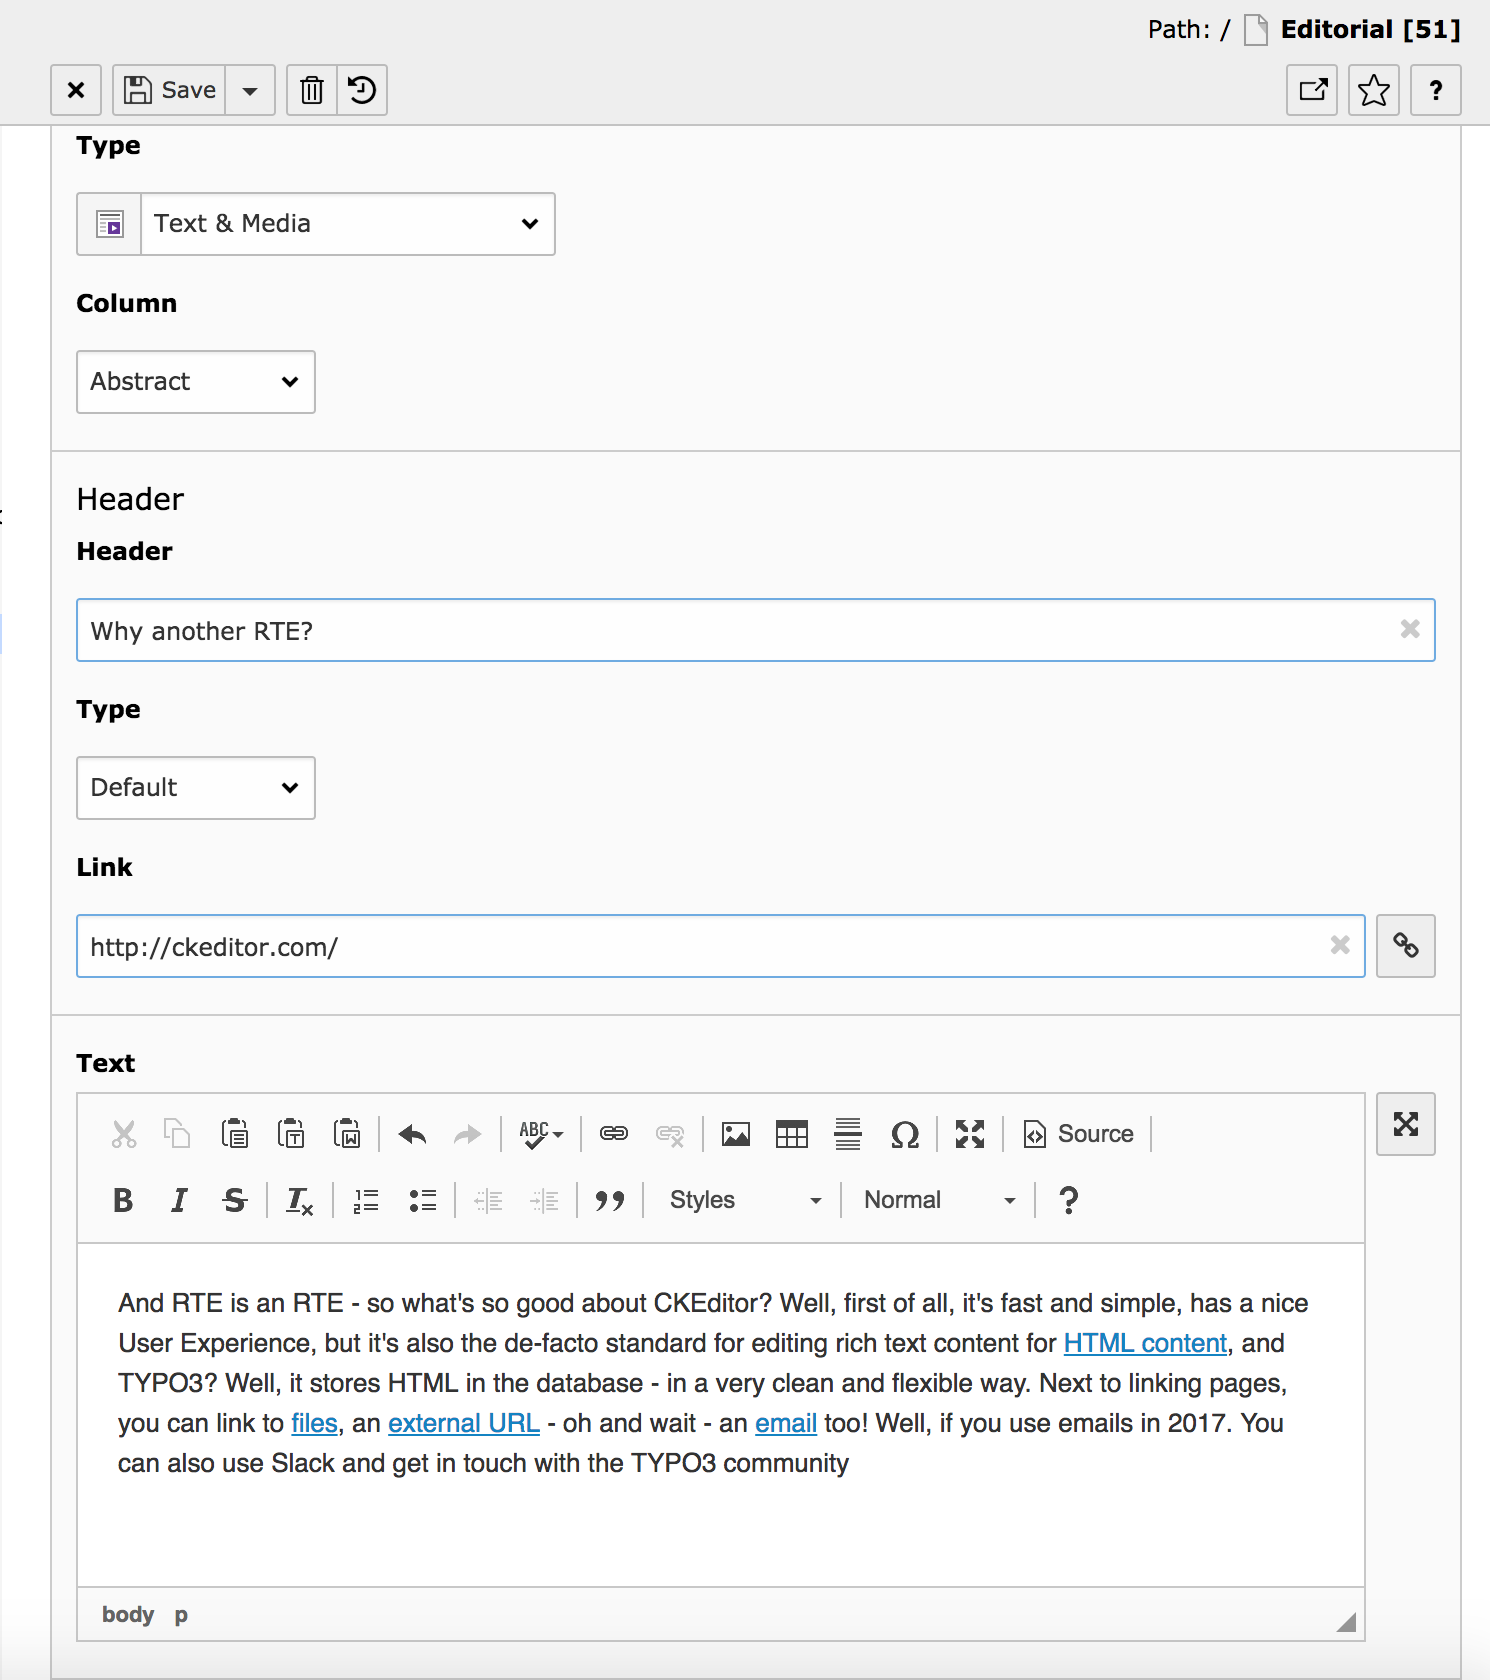
\includegraphics[width=0.8\linewidth]{BackendUserInterface/ckeditor.png}
			\end{figure}
		\end{column}
	\end{columns}

\end{frame}



% ------------------------------------------------------------------------------
% LTXE-SLIDE-START
% LTXE-SLIDE-UID:		c9dc360d-cf218f95-03f53731-03d821ad
% LTXE-SLIDE-TITLE:		#78383: Field positions in tabs streamlined (TCA)
% ------------------------------------------------------------------------------
\begin{frame}[fragile]
	\frametitle{Interface Utilisateur Backend}
	\framesubtitle{Position et ordre des éléments}

	\begin{itemize}
		\item L'ordre et la position de certains champs du backend TYPO3 ont été rationalisés
		\item Le but est de satisfaire l'attente des utilisateurs sur l'emplacement des
			options communes dans l'interface utilisateur
		\item Particulièrement important pour les définitions de champs récurrents et les
			catégories génériques partagées par de nombreux enregistrements
		\item Les auteurs d'extension sont encouragés à suivre les positions et ordres des éléments
			spécifiés dans la \href{https://docs.typo3.org}{documentation officelle}

			% TODO: update link above (waiting for Doc and Core Team to finish documentation)

	\end{itemize}

	\begin{itemize}
		\item \textit{La cohérence du backend est primordiale~!} :-)
	\end{itemize}

\end{frame}

% ------------------------------------------------------------------------------
